\documentclass[11pt]{amsart}

% packages

\usepackage{amsfonts, amsthm, amssymb, amsmath, stmaryrd, etoolbox, mathtools}
\usepackage{graphicx,caption,subcaption}
\usepackage{tikz}
\usetikzlibrary{matrix,arrows}

% new commands

\newcommand{\RR}{\mathbb{R}}
\newcommand{\ZZ}{\mathbb{Z}}
\newcommand{\NN}{\mathbb{N}}
\newcommand{\QQ}{\mathbb{Q}}
\newcommand{\CC}{\mathbb{C}}
\newcommand{\from}{\colon}
\newcommand{\defn}[1]{\textbf{#1}}
\newcommand{\tin}{\colon}

% fonts

\newcommand{\cat}[1]{\mathbf{#1}}
\newcommand{\type}[1]{\mathtt{#1}}

% math operators

\DeclareMathOperator{\Hom}{Hom}
\DeclareMathOperator{\id}{id}
\DeclareMathOperator{\ob}{Ob}
\DeclareMathOperator{\arr}{arr}
\DeclareMathOperator{\im}{im}
\DeclareMathOperator{\Aut}{Aut}
\DeclareMathOperator{\Bij}{Bij}
\DeclareMathOperator{\Sub}{Sub}

%%%%%%%%%%%%%
% begin document
%%%%%%%%%%%%%
\begin{document}

\title{Notes on a pushout of sets}
\maketitle

%%%%%%%%%%%%%
% new section
%%%%%%%%%%%%%
\section{the setup}

The idea is that we have types $A$, $B$, and $C$, all of which are sets. 
The question: is the pushout given by the square
\[
	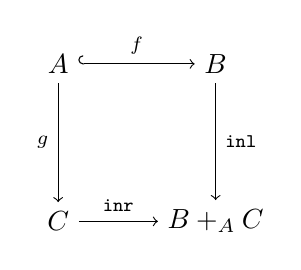
\begin{tikzpicture}
		\node (C) at (0,0) {$C$};
		\node (BAC) at (2,0) {$B +_A C$};
		\node (A) at (0,2) {$A$};
		\node (B) at (2,2) {$B$};
		\draw[right hook ->]  (A) to node [above] {\scriptsize $f$} (B);
		\draw[->]  (A) to node [left] {\scriptsize $g$} (C);
		\draw[->]  (B) to node [right] {\scriptsize $\type{inl}$} (BAC);
		\draw[->]  (C) to node [above] {\scriptsize $\type{inr}$} (BAC);
	\end{tikzpicture}
\]
also a set when $f$ is a monomorphism?

Recall that a \defn{set} is a type such that, 
for any elements $x$, $y$ and $p$, $q \from x = y$, 
we have $p = q$.  
Thus to determine whether $B +_A C$ is a set,
we need to access its identity types.  
We do this with an \emph{encode-decode} style proof.  

Roughly, a proof of this sort begins by guessing
what the identity types are.  That is,
for each $x$ and $y$ in $B +_A C$, 
we define a type 
\[
	\type{code} \from B +_A C \to B +_A C \to \type{Type}
\]
so that $\type{code}(x,y)$ serves as our guess  
as to what $x =_{\scriptsize B +_A C} y$ actually is.  
Then we define functions
\[
	\type{ encode }_{ x , y } \from  ( x = y ) \to \type{code} ( x , y ) 
	\text{ and }
	\type{ decode }_{ x , y } \from \type{code} ( x , y ) \to ( x = y )
\]
for each $x$ and $y$ in $B +_A C$.  
Hopefully, these are mutually inverse.

%%%%%%%%%%%%%
% new section
%%%%%%%%%%%%%
\section{defining $\type{code}$}

Let's try to define 
$\type{code} \from B +_A C \to B +_A C \to \type{Type}$.  
Note that $\type{code}$ is a map from a coproduct, 
so we can define it using induction of higher types.
This requires us to define, at first, three types schemes:
\begin{align*}
	\type{code}(\type{inl}(b)) & \from B +_A C \to \type{Type} \\
	\type{code}(\type{inr}(c)) & \from B +_A C \to \type{Type} \\
	\type{code}(\type{ap_{glue}}(a)) & \from B +_A C \to \type{Type} \\
\end{align*}
These run through $a \tin A$, $b \tin B$, and $c \tin C$.  
But these are also functions on the same coproduct!
To define $\type{code}(\type{inl}(b))$, 
we use higher induction which gives the type schemes:
\[
	\type{code}(\type{inl}(b),\type{inl}(b')), \hspace{0.5em}
	\type{code}(\type{inl}(b),\type{inr}(c')), \hspace{0.5em}
	\type{code}(\type{inl}(b),\type{ap_{glue}}(a')).
\]
Similarly, we define $\type{code}(\type{inr}(c))$ by
\[
	\type{code}(\type{inr}(c),\type{inl}(b')), \hspace{0.5em}
	\type{code}(\type{inr}(c),\type{inr}(c')) , \hspace{0.5em}
	\type{code}(\type{inr}(c),\type{ap_{glue}}(a')).
\]
and $\type{code}(\type{glue}(a))$ by 
\[
	\type{code}(\type{ap_{glue}}(a),\type{inl}(b')), \hspace{0.5em}
	\type{code}(\type{ap_{glue}}(a),\type{inr}(c')) , \hspace{0.5em} 
	\type{code}(\type{ap_{glue}}(a),\type{ap_{glue}}(a')).
\]
The $\type{code}$'s that have 
no $\type{ap_{glue}}$'s in the arguments 
correspond to our guesses
for the identity types.
The $\type{code}$'s that have 
one $\type{ap_{glue}}$ in the arguments
give a pre- or post-composition
of paths.
The $\type{code}$'s that have 
two $\type{ap_{glue}}$'s in the arguments  
ensure that this pre- and post-composition
action is coherent.
This fits together in a nice little 
diagram:
\[
	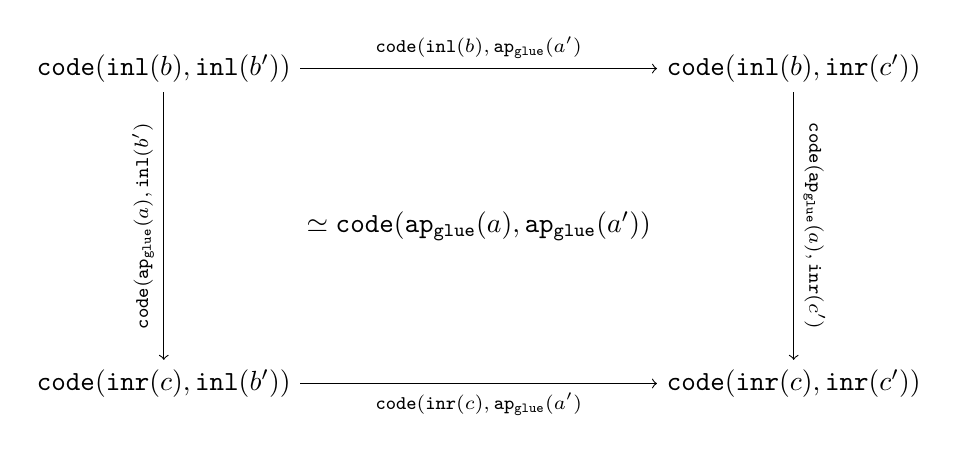
\begin{tikzpicture}
		\node (AA) at (0,0) 
			{ $ \simeq \type{ code } ( \type{ ap_{glue} } ( a ) , \type{ ap_{glue} } ( a' )  )$ }; 
		\node (BB) at (-4,2) 
			{ $ \type{ code } ( \type{ inl } ( b ) , \type{ inl } ( b' )  )$ }; 
		\node (BC) at (4,2) 
			{ $ \type{ code } ( \type{ inl } ( b ) , \type{ inr } ( c' )  )$ }; 
		\node (CB) at (-4,-2) 
			{ $ \type{ code } ( \type{ inr } ( c ) , \type{ inl } ( b' )  )$ }; 
		\node (CC) at (4,-2) 
			{ $ \type{ code } ( \type{ inr } ( c ) , \type{ inr } ( c' )  )$ }; 
		\draw [->] (BB) to 
			node 
				[above] 
				{\scriptsize $ \type{ code } ( \type{ inl } ( b ) , \type{ ap_{glue} } ( a' ) $ } 
			(BC);
		\draw [->] (BB) to 	
			node 
				[rotate=90,above] 
				{ \scriptsize $ \type{ code } ( \type{ ap_{glue} } ( a ) , \type{ inl } ( b' ) $ } 
			(CB);
		\draw [->] (BC) to 
			node 
				[rotate=-90, above] 
				{\scriptsize $\type{ code } ( \type{ ap_{glue} } ( a ) , \type{ inr } ( c' ) $} 
			(CC);
		\draw [->] (CB) to 	
			node 
				[below] 
				{ \scriptsize $ \type{ code } ( \type{ inr } ( c ) , \type{ ap_{glue} } ( a' ) $ } 
			(CC);
	\end{tikzpicture}
\]
Next, let's define all of these $\type{code}$'s.





%%%%%%%%%%%%%
% end document
%%%%%%%%%%%%%
\end{document}
